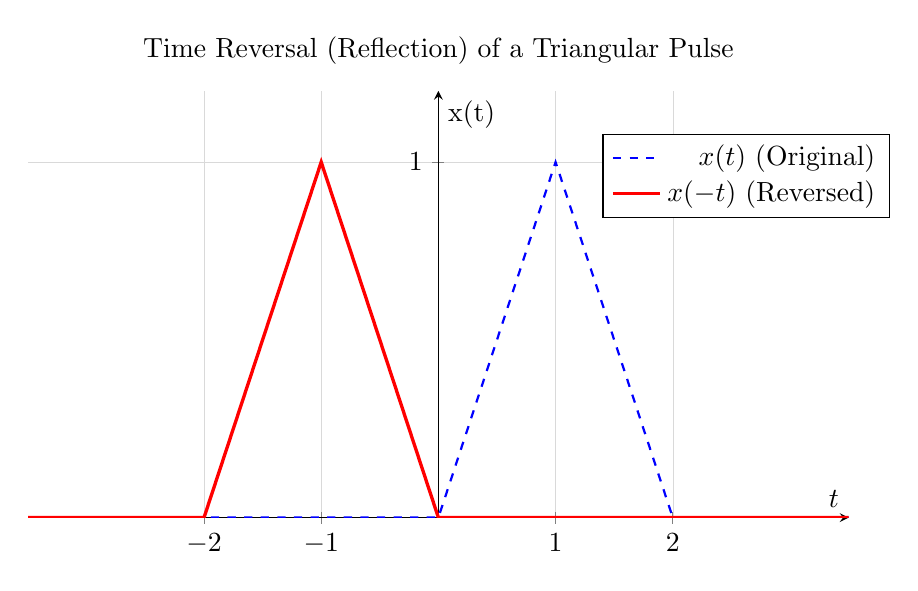
\begin{tikzpicture}
	\begin{axis}[
		% Set the overall style
		width=12cm,
		height=7cm,
		% Title describing the transformation
		title={Time Reversal (Reflection) of a Triangular Pulse},
		% Axis labels
		xlabel={$t$},
		ylabel={x(t)},
		% Position axes at the origin
		axis lines=middle,
		% Set axis limits to show both signals
		xmin=-3.5, xmax=3.5,
		ymin=0, ymax=1.2,
		% Set ticks at key points for both signals
		xtick={-2, -1, 1, 2},
		ytick={1},
		yticklabels={$1$},
		% Add a grid
		grid=major,
		grid style={line width=.1pt, draw=gray!30},
		% Position the legend
		legend style={
			at={(0.7, 0.9)}, % 3% from left, 97% from bottom
			anchor=north west,   % Anchor the top-left corner of the legend
			legend cell align={right}
		},
		]
		
		% 1. Plot the original signal (dashed blue) for reference
		\addplot[blue, dashed, thick] coordinates {
			(-3.5,0) (0,0) (1,1) (2,0) (3.5,0)
		};
		\addlegendentry{$x(t)$ (Original)};
		
		% 2. Plot the time-reversed signal (solid red)
		\addplot[red, very thick] coordinates {
			(-3.5,0) (-2,0) (-1,1) (0,0) (3.5,0)
		};
		\addlegendentry{$x(-t)$ (Reversed)};
		
	\end{axis}
\end{tikzpicture}